% \documentclass{article}
% \usepackage{amsmath,amssymb}
% \DeclareMathOperator{\E}{\mathbb{E}} % For the expectation style E
% \usepackage{graphicx}
% \usepackage{tabularx}
% \usepackage[a4paper, total={6.5in, 10in}]{geometry} % Set margin size.
% \usepackage[framed,numbered,autolinebreaks,useliterate]{mcode}
% \usepackage{titlesec}

% \setcounter{tocdepth}{4} % Sets table of contents depth to 4 sections.
% \setcounter{secnumdepth}{4} % Sets document depth to 4 sections.
% \titleformat{\paragraph}
% {\normalfont\normalsize\bfseries}{\theparagraph}{1em}{}
% \titlespacing*{\paragraph}
% {0pt}{3.25ex plus 1ex minus .2ex}{1.5ex plus .2ex}


% \begin{document}


\section{Random Signals and Stochastic Processes}
\vspace{0.5cm}

\subsection{Statistical Estimation}

We generate a vector $\bf x$ containing 1000 samples from a Uniform Distribution $U(0,1)$, and observe its plot shown in Figure \ref{fig:mean_norm}. 

\begin{figure}[h!]
\centering
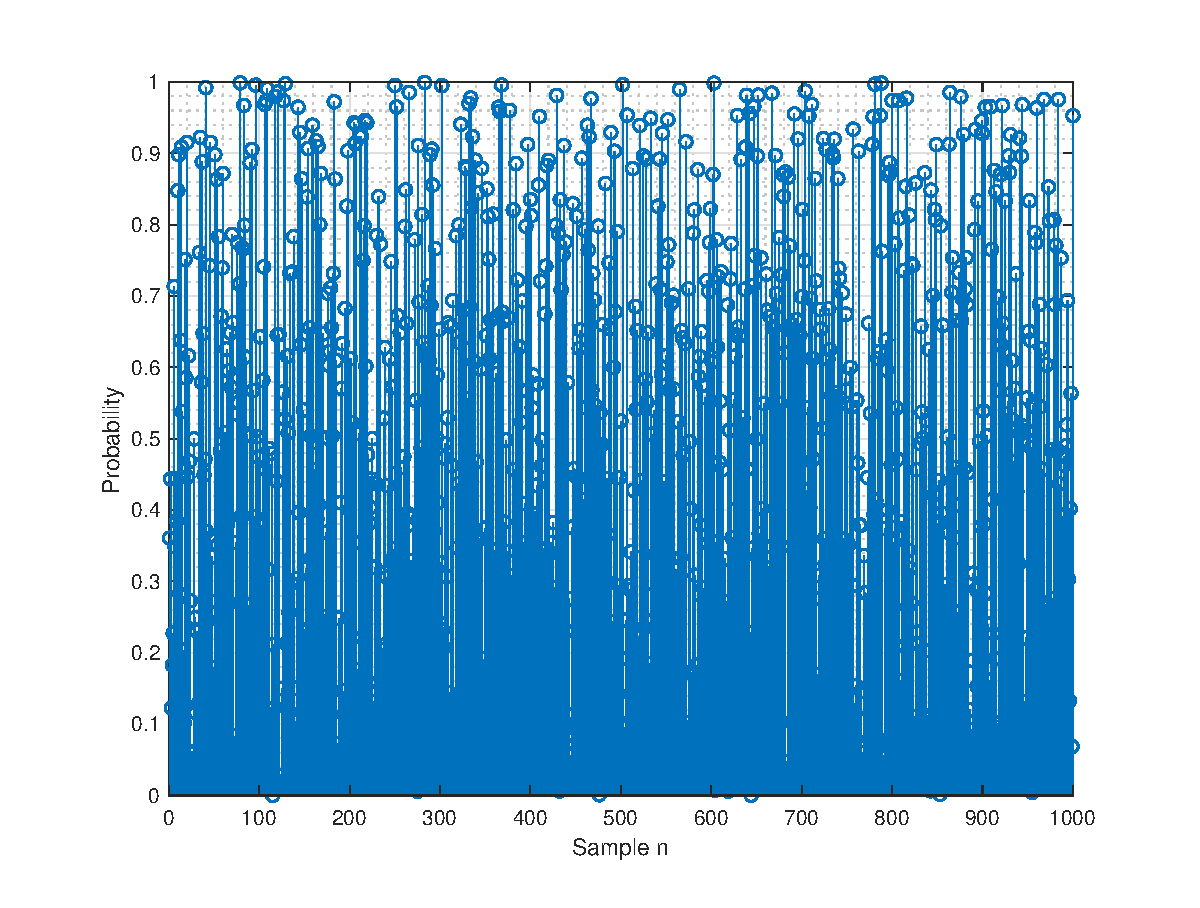
\includegraphics[width=0.5\textwidth]{mean_norm}
\caption{\label{fig:mean_norm} 1000 samples of a Uniform Distribution $U(0,1)$}
\end{figure}

\subsubsection{Sample and Theoretical Mean}

We know that the \textit{theoretical mean} is $0.5$ since we are given a uniform probability distribution between 0 and 1. We calculate the \textit{sample mean} using $\bf x$. Since the accuracy of the estimator increases with more samples, there will be a certain error in the mean calculated by this method.

\begin{table}[h!]
\centering
\begin{tabular}{|l|r|} \hline

Sample Mean	&Error \\ \hline
0.49683		&0.0031684	\\ \hline
0.49296		&0.0070372	\\ \hline
0.49018		&0.0098166	\\ \hline
0.50179		&-0.001792 \\ \hline
0.50605		&-0.0060459	\\ \hline
\end{tabular}
\end{table}

Thus we see that the sample mean matches the theoretical mean up to 2 decimal places.

\subsubsection{Sample and Theoretical Standard Deviation}

The \textit{theoretical standard deviation} converges to $0.28868$. Multiple iterations give the following values for \textit{sample standard deviation}:

\begin{table}[h!]
\centering
\begin{tabular}{|l|r|} \hline

Sample Standard Deviation	&Error \\ \hline
0.29143						&-0.0027575	\\ \hline
0.2938						&-0.005121	\\ \hline
0.28912						&-0.00044826	\\ \hline
0.28221						&0.0064643 \\ \hline
0.28569						&0.002981	\\ \hline
\end{tabular}
\end{table}

The sample standard deviation shows the same level of accuracy as the mean, with theoretical and sample values being identical up to 2 decimal places.

\pagebreak

\subsubsection{Bias Estimation}

The estimator bias for the mean and standard deviation for 10 realizations of $\bf x$, each having 1000 samples, are shown in Figure \ref{fig:bias_norm}.

\begin{figure}[h!]
\centering
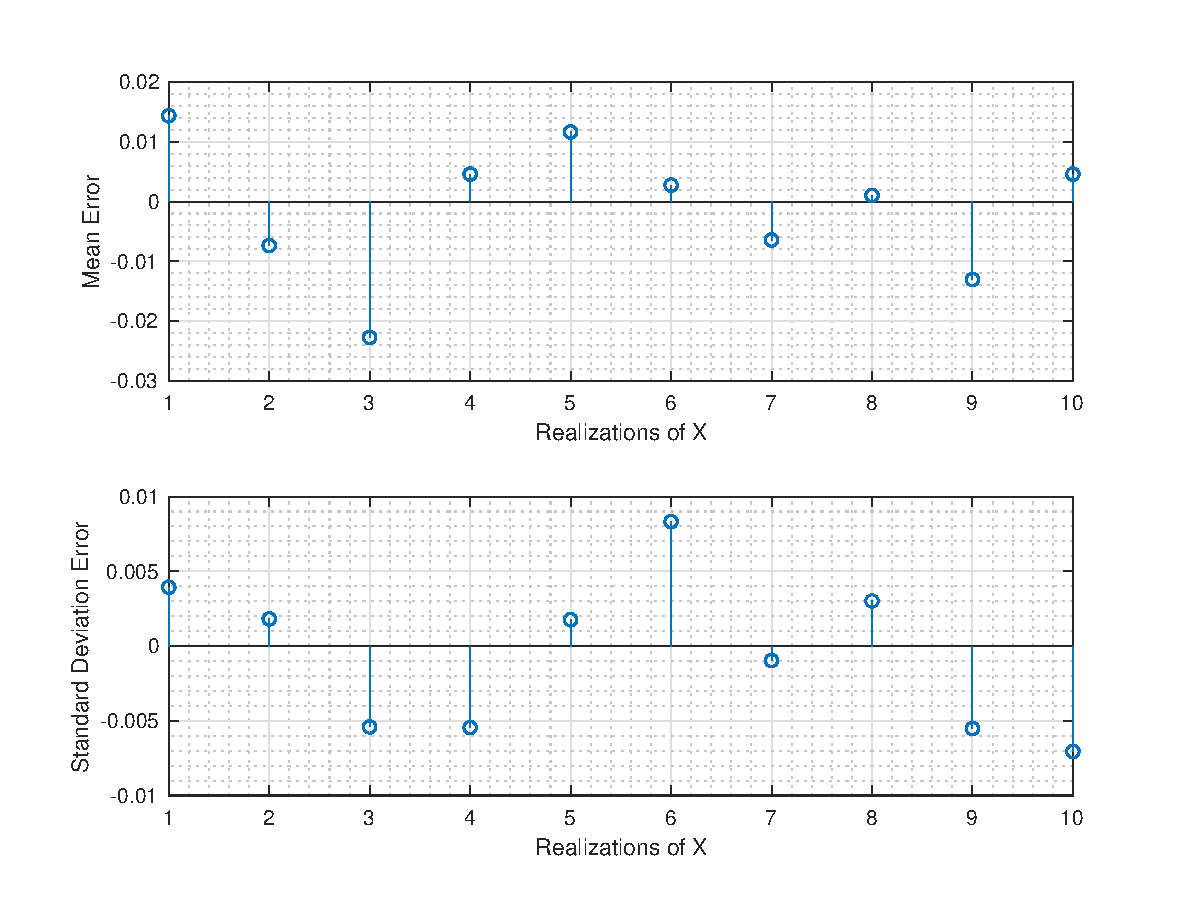
\includegraphics[width=0.6\textwidth]{bias_norm}
\caption{\label{fig:bias_norm} Bias of mean and standard deviation. Bias given by $B = E[X]-m$}
\end{figure}


\subsubsection{Estimating the Probability Density Function}
\label{sec:1.1.4}

Since the histogram in Figure \ref{fig:pdf_norm} has 10 bins, each bin's probability must tend to 0.1 since the total theoretical probability is 1. The accuracy of the estimation increases as you increase the number of samples, i.e, the probability of each bin becomes closer to $0.1$.

\begin{figure}[h!]
\centering
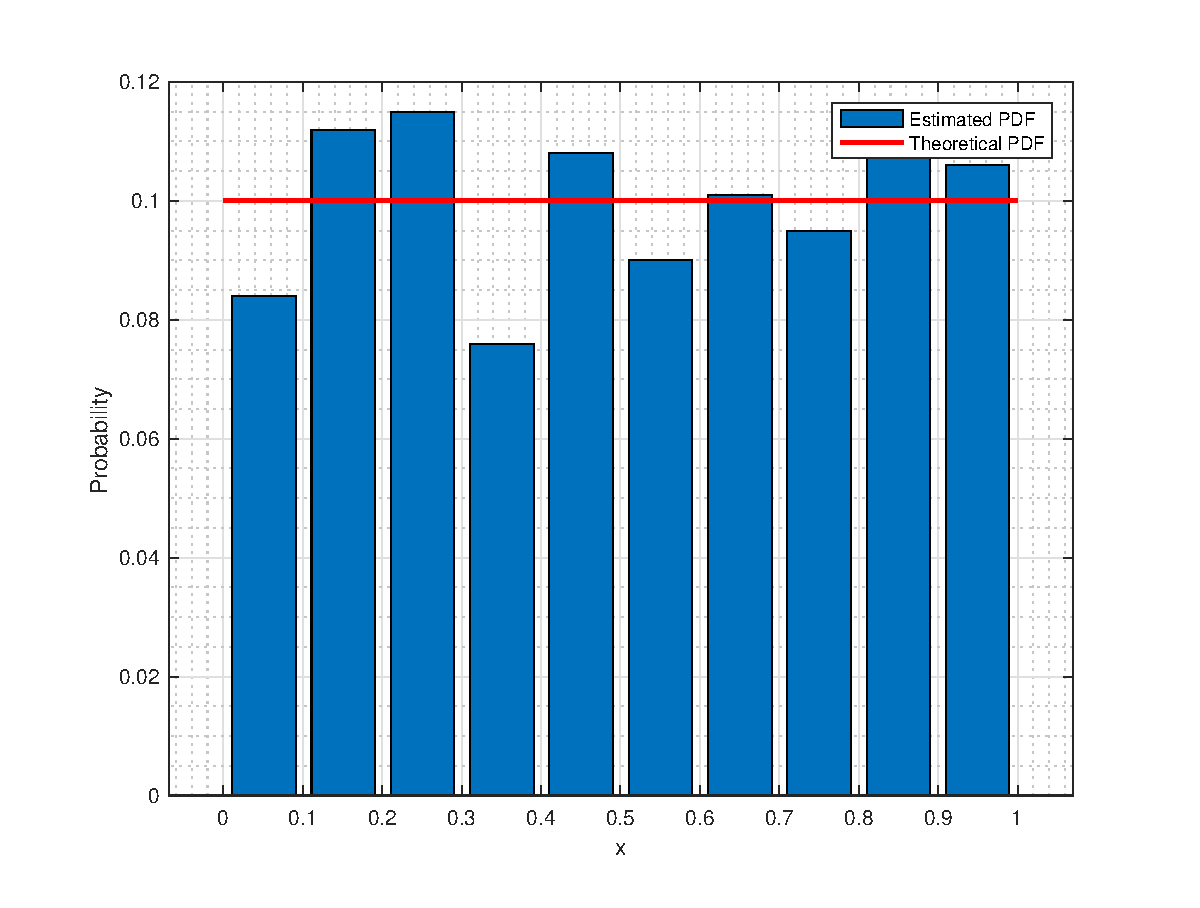
\includegraphics[width=0.5\textwidth]{pdf_norm}
\caption{\label{fig:pdf_norm} Estimated PDF for 1000 samples from $U(0,1)$}
\end{figure}


\subsubsection{Using a Gaussian Random Variable}

We now use Gaussian random variables instead of Uniform ones, and repeat our analysis.\\

The \textit{theoretical mean} of the new Gaussian distribution is 0 and the \textit{theoretical standard deviation} is 1. The estimated values of the mean and standard deviation lie close to their theoretical values, and we can observe the bias for 10 iterations of the random variable in Figure \ref{fig:bias_gaussian}.\\

\begin{figure}[h!]
\centering
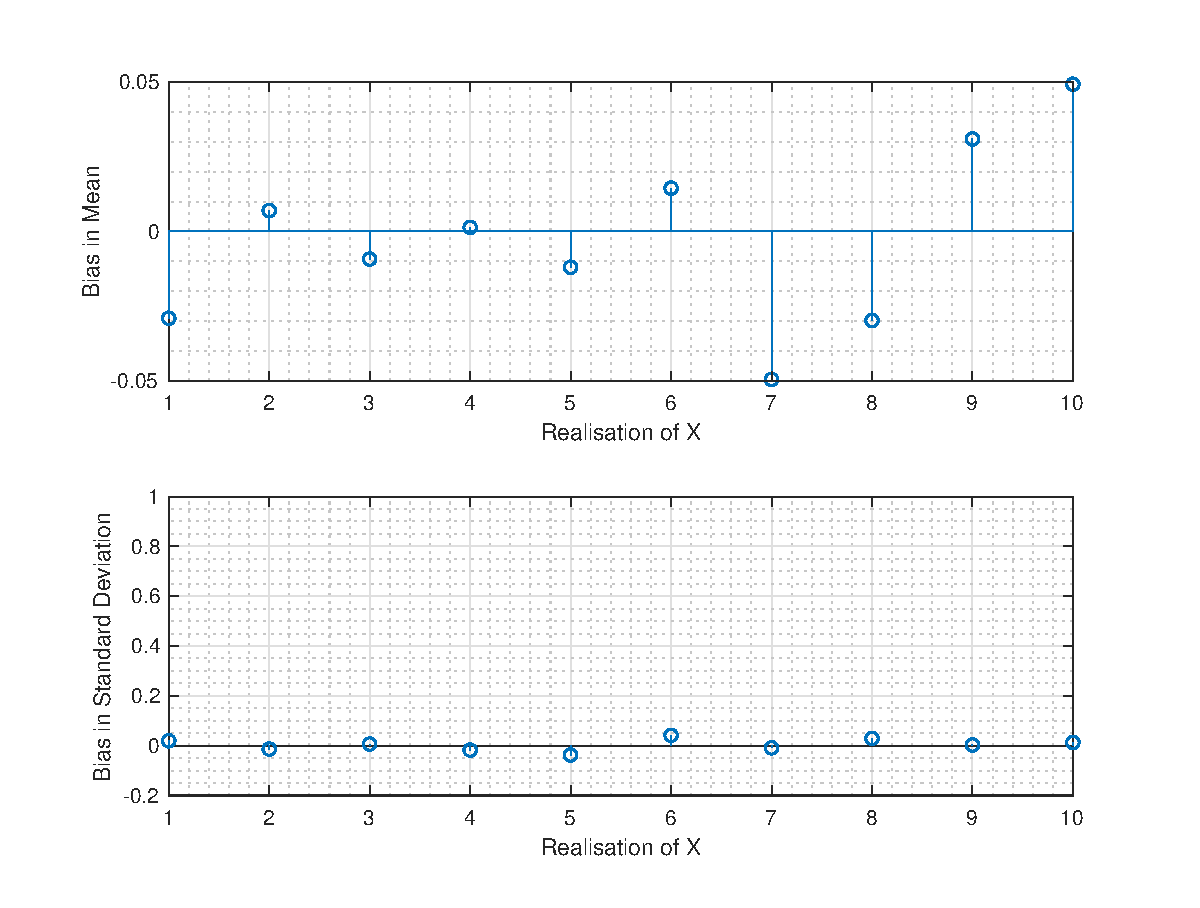
\includegraphics[width=0.6\textwidth]{bias_gaussian}
\caption{\label{fig:bias_gaussian} Bias in mean and standard deviation for 10 Gaussian random variables}
\end{figure}

An estimate of the probability density function can be derived using the same program as before. The output for 10,000 samples is shown in Figure \ref{fig:pdf_gaussian}.

\begin{figure}[h!]
\centering
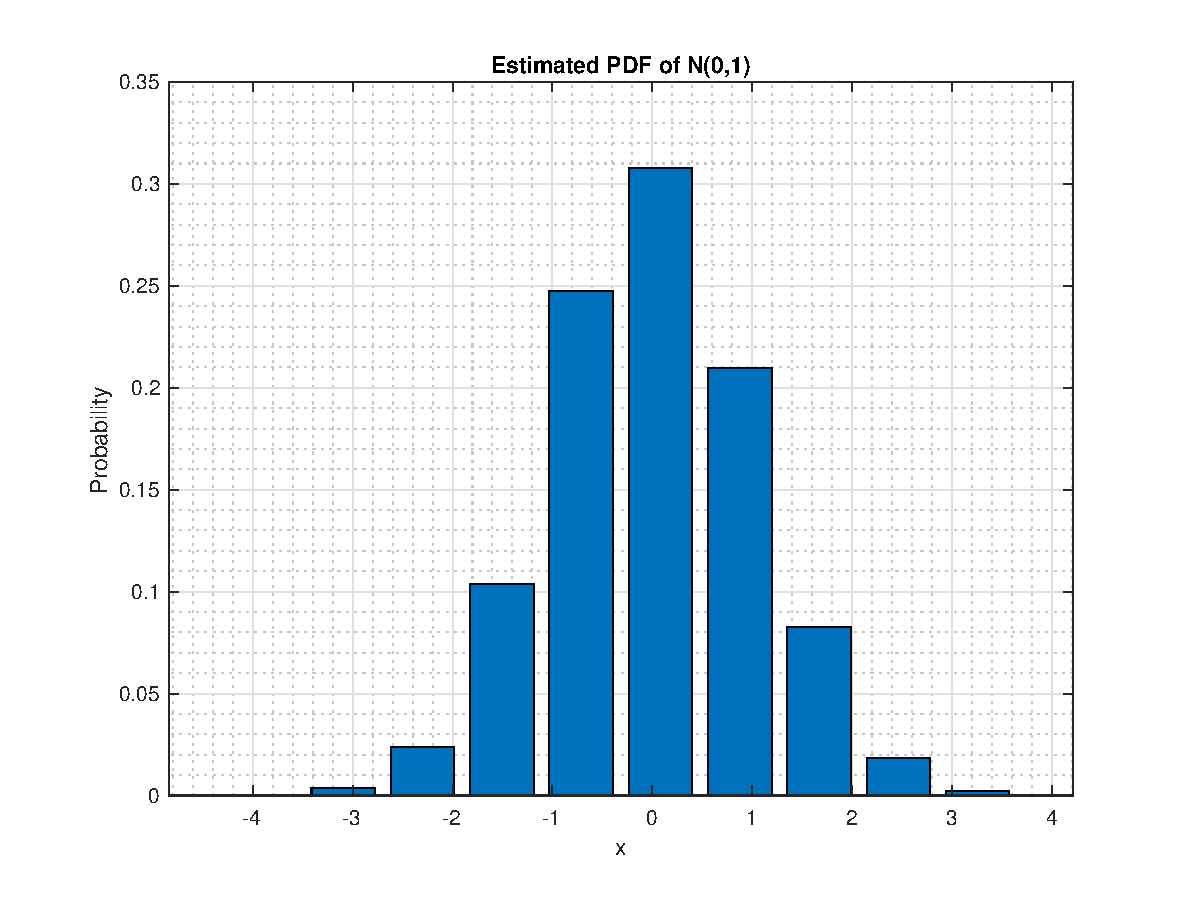
\includegraphics[width=0.5\textwidth]{pdf_gaussian}
\caption{\label{fig:pdf_gaussian} Estimated PDF for 10,000 samples of $N(0,1)$}
\end{figure}


\pagebreak

\subsection{Stochastic Processes}

\begin{itemize}
\item A \textit{stochastic} or random process is defined as a collection of random variables.

\item A \textit{stationary} process is a random process whose statistical properties - such as its mean, moments and variance - remain constant over time.

\item An \textit{ergodic} process is one in which the \textit{time average equals the ensemble average}. This means that you get the same result if you measure statistical properties of one ensemble member over the entire time period or of all ensemble members at one time instant.
\end{itemize}

We are given 3 random processes to analyze - $rp1$, $rp2$ and $rp3$. Each of the 3 Matlab functions that generate these processes outputs an $M$ by $N$ matrix, where $M$ is the number of ensemble members and $N$ is the number of samples in each ensemble. Using the \textit{plot} function graphs the data points in a column against the column number.

\pagebreak

\subsubsection{Ensemble Mean and Standard Deviation}

Figure \ref{fig:ergodic_rp1} shows that $rp1$ is not stationary since both its mean and standard deviation vary over time. The mean for the given signal is linearly increasing and can be approximated by the equation $mean = \frac{t}{50}$, where $t$ is the sample number. The standard deviation can be described by the equation $$ SD = 1.44 \ sin(\frac{t\pi}{T})$$ where $t$ is as before and $T$ is the total number of samples.\\

\begin{figure}[h!]
\centering
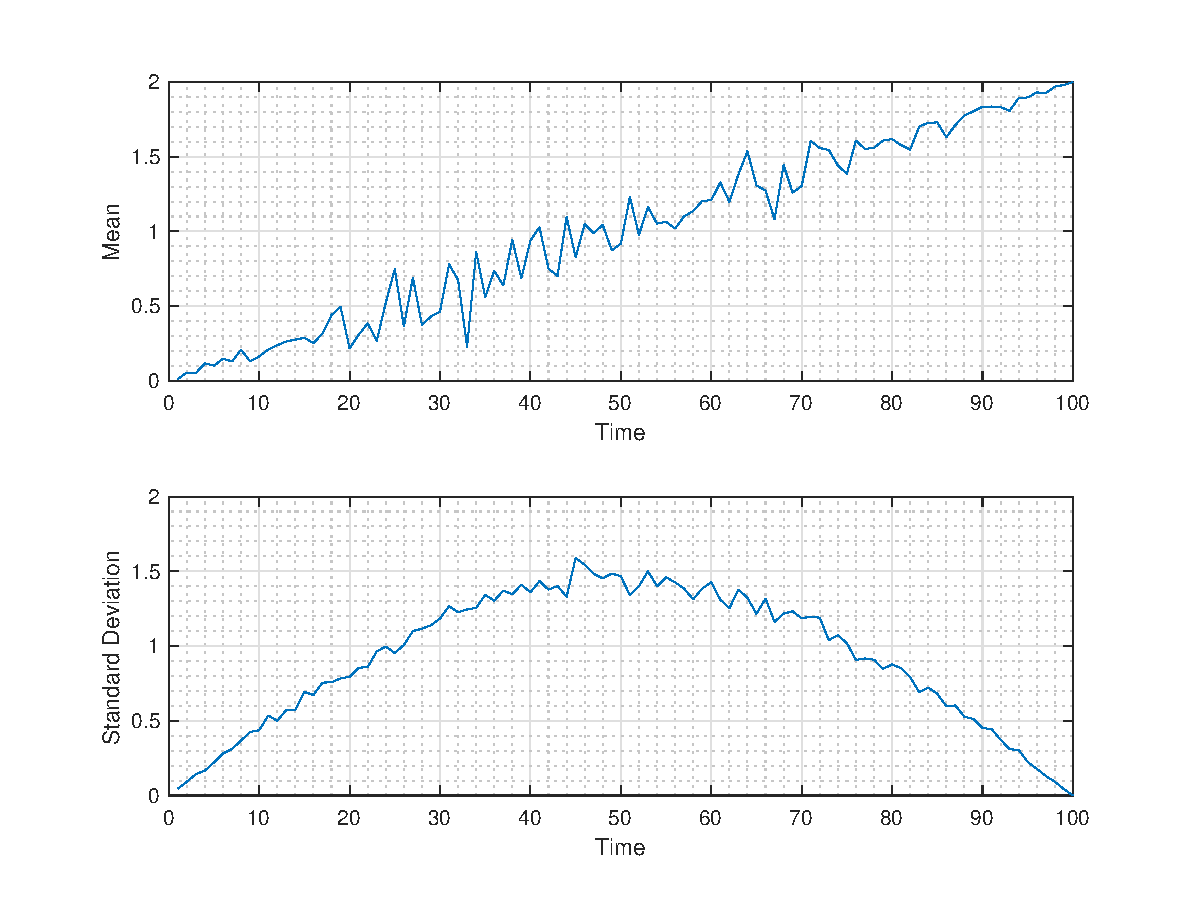
\includegraphics[width=0.65\textwidth]{ergodic_rp1}
\caption{\label{fig:ergodic_rp1} Mean and standard deviation of $rp1$ with respect to time}
\end{figure}

Figure \ref{fig:ergodic_rp2} and Figure \ref{fig:ergodic_rp3} show that $rp2$ and $rp3$ respectively are both stationary. $rp2$ has a constant mean of $0.53$ and standard deviation of $0.34$. $rp3$ has a constant mean of $0.5$ and $0.87$. These can be checked by further increasing $M$ and $N$.

\begin{figure}[h!]
\centering
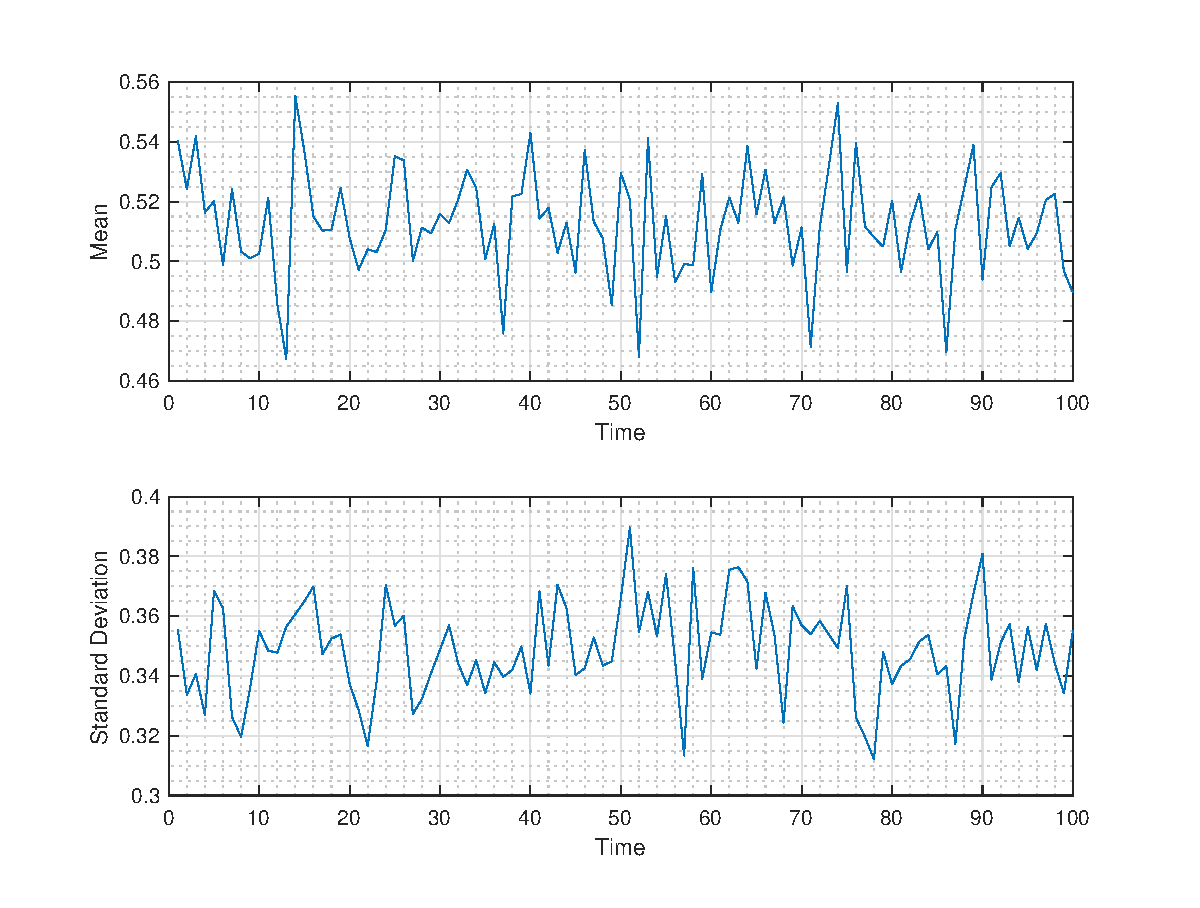
\includegraphics[width=0.65\textwidth]{ergodic_rp2}
\caption{\label{fig:ergodic_rp2} Mean and standard deviation of $rp2$ with respect to time}
\end{figure}

\begin{figure}[h!]
\centering
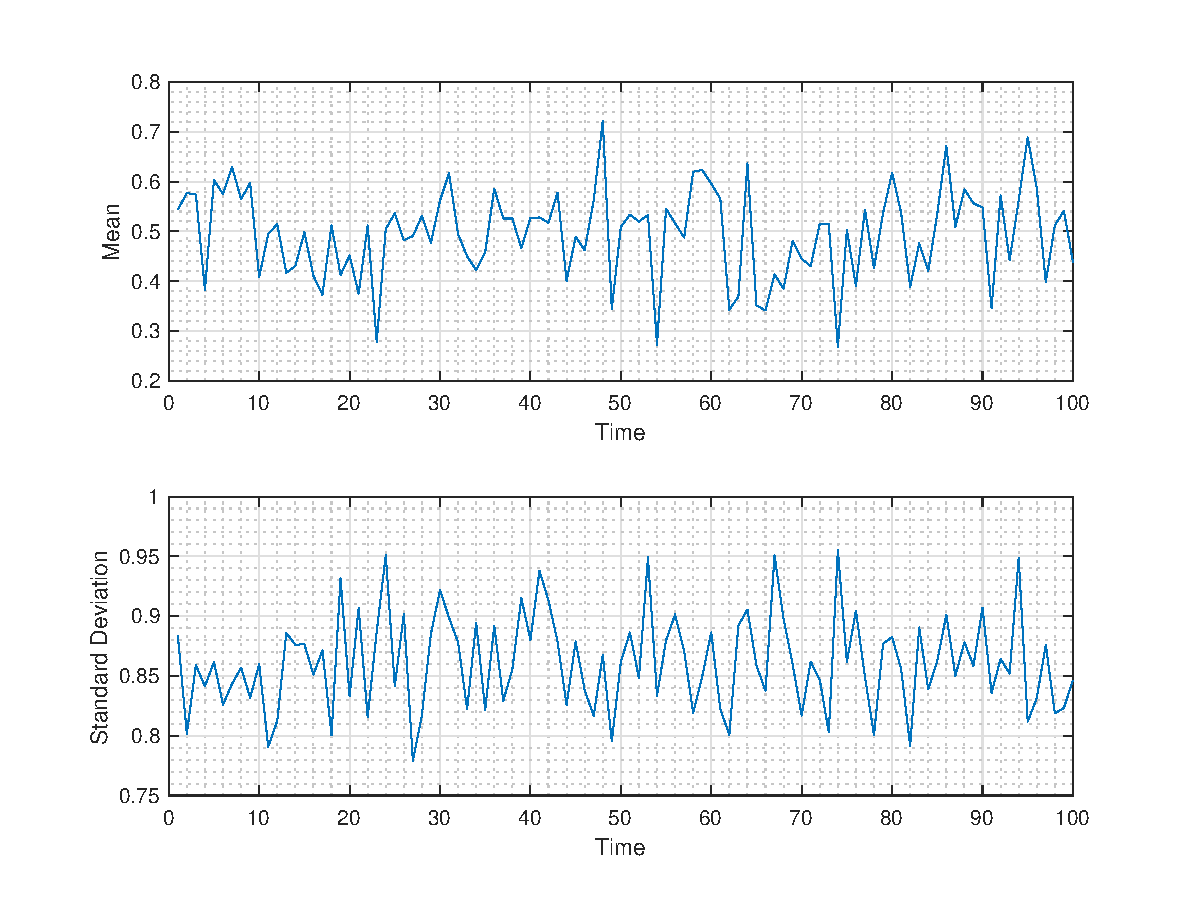
\includegraphics[width=0.65\textwidth]{ergodic_rp3}
\caption{\label{fig:ergodic_rp3} Mean and standard deviation of $rp3$ with respect to time}
\end{figure}

\pagebreak
\subsubsection{Ergodicity when $M=4$ and $N=1000$}

We now have 4 samples at 1000 different moments of time. In other words, 1000 realizations of 4 samples.\\

$rp1$ cannot be ergodic because its ensemble mean is linearly increasing with time, and therefore the ensemble average cannot equal the time average for all time. This means that examining multiple ensembles at one point in time will not reveal the properties of the signal completely.\\

$rp2$ is not ergodic either. Each set of 4 samples for every time point provides different values of mean and standard deviation, which can be observed in Table \ref{fig:rp2}. This means that the system's properties cannot be gleaned from analyzing all ensembles at a single point in time.\\

\begin{table}[h!]
\centering
\begin{tabular}{|l|r|r|} \hline

Trial	&Expectation of Mean	&Expectation of Standard Deviation \\ \hline
1		&0.2630					&0.3411	\\ \hline
2		&0.7350					&0.2902	\\ \hline
3		&0.5625					&0.2404	\\ \hline
4		&0.5309					&0.2292 \\ \hline
5		&0.6480					&0.3091	\\ \hline
\end{tabular}
\caption{\label{fig:rp2} Variations of mean and standard deviation of $rp2$}
\end{table}

$rp3$ is ergodic since it has a constant mean and standard deviation over all time. Therefore analyzing all ensembles at one point in time can provide accurate information about the entire process.

\pagebreak

\subsubsection{A Mathematical Description of the Mean and Standard Deviation}

\paragraph{rp1}

$rp1$ is defined as

\begin{equation}
v_t=cb \times \sin(\frac{t\pi}{T})+at
\end{equation}

where $a=0.02$, $b=5$ and $c\sim U(-0.5,0.5)$. Therefore $E[c]=0$ and $Var(c)=\frac{1}{12} \Rightarrow \sigma_c=\frac{1}{\sqrt[]{12}}$. $t$ represents the particular sample and $T$ is the total number of samples.

\begin{equation}
E[v_t]=E[cb \times \sin(\frac{t\pi}{T})+at]=E[c] \times E[b \times \sin(\frac{t\pi}{T})]+E[at]=0+E[at]=aE[t]=at=\frac{t}{50}
\end{equation}

\begin{align} % Remember to put &= for all equal signs that you want to align
Var(v_t) &= E[v_t^2]-E[v_t]^2 = E[c^2b^2sin^2(\frac{t\pi}{T})+a^2t^2+2cb\sin(\frac{t\pi}{T})at]-a^2t^2 \\
&= E[c^2b^2sin^2(\frac{t\pi}{T})]+E[a^2t^2]-a^2t^2 \\
&= E[c^2] \times b^2sin^2(\frac{t\pi}{T}) \\
&= \frac{1}{12} \times b^2sin^2(\frac{t\pi}{T}) \\
\end{align}

Note that we have found $E[c^2]$ using $Var(c)=E[c^2]-E[c]^2$. We now have

\begin{equation}
\sigma_{v_t}=\sqrt[]{Var(v_t)}=\frac{1}{\sqrt[]{12}}b\sin(\frac{t\pi}{T})=1.44 \times \sin(\frac{t\pi}{T})
\end{equation}

Thus both the mean and standard deviation of $rp1$ match what was observed in Section 1.2.1.


\paragraph{rp2}

$rp2$ is defined by Equation \ref{eq:rp2}. Note that the random variable $Z$ is derived from a matrix with $M \times N$ distinct random numbers, and therefore depends on both the ensemble members as well as the sample instance. $X$ and $Y$ on the other hand only depend on the sample instance.

\begin{equation} % Use \times for multiplication cross
\label{eq:rp2}
v_t = X_n + Y_n \times Z_{n,t}
\end{equation}

$X$ and $Y$ are simply randomly distributed numbers between $0$ and $1$, so $E[X_n]$ and $E[Y_n]$ both equal $0.5$. The standard deviation is $\sigma_{X_n}=\sqrt[]{Var(X_n)}=\frac{1}{\sqrt[]{12}}$.\\

Since $Z_n$ is randomly distributed between $-0.5$ and $0.5$, $E[Z_n]=0$. Its standard deviation is also $\frac{1}{\sqrt[]{12}}$ since it is a uniform distribution spanning a length of 1. Therefore

\begin{equation}
E[v_t]=E[X_n]+E[Y_n] \times E[Z_n] =E[X_n]+E[Y_n] \times 0=E[X_n] \Rightarrow X_n \rightarrow 0.5
\end{equation}

This means that although a single realization of $rp2$ has a random mean, the mean tends to 0.5 for over many realizations.\\

The standard deviation of $rp2$ is

\begin{align}
Var(v_t) = E[v_t^2]-E[v_t]^2 &=E[X_n^2 + 2X_n Y_n \times Z_{n,t} + Y_n^2Z_n^2]-X_n^2\\
&= E[X_n^2]+E[Y_n^2]E[Z_{t,n}^2]-X_n^2
\end{align}

since $E[Z_{t,n}]=0$. $E[X_n^2]$ can be found from $Var(X_n)=E[X_n^2]-E[X_n]^2$, which gives $E[X_n^2]=\frac{1}{12} + 0.25 = 0.333$. Similarly $E[Y_n]=0.333$ and $E[Z_{t,n}^2]=\frac{1}{12}$.

\begin{equation}
\sigma_{v_t}=\sqrt[]{Var(v_t)}=\sqrt[]{0.333 + (0.333 \times \frac{1}{12}) - 0.25}=0.333
\end{equation}

Thus both the mean and standard deviation of $rp2$ match what was observed in Section 1.2.1.


\paragraph{rp3}

$rp3$ is defined as

% Use \text{} to insert text in between equations
% Use \cdot for multiplication dot
\begin{equation}
v_t=m\cdot X +a \text{, where } X=U(-0.5\text{, }0.5)\text{, }m=3\text{, and }a=0.5
\end{equation}

Therefore its expected value is

\begin{equation}
E(v_t)=m \cdot E(X)+a=0+a=a=0.5
\end{equation}

and its standard deviation is

\begin{equation}
Var(v_t)=E[v_t^2]-E[v_t]^2=E[m^2x^2+a^2+2 \cdot amX] - 0.25 = 0.75
\end{equation}

% Use \approx for approximately equal sign
\begin{equation}
\sigma_{v_t}=\sqrt[]{Var(v_t)}=\sqrt[]{0.75} \approx 0.87
\end{equation}

Thus both the mean and standard deviation of $rp3$ match what was observed in Section 1.2.1.


\vspace{0.5cm}
\subsection{Estimation of Probability Distributions}

\subsubsection{For a stationary process}

The following code has been used to implement the PDF estimator:

\begin{lstlisting}
N = 10000;
v = randn(1,N);
[freq,bin] = hist(v,100); % Returns frequency and centre of each bin.
freq = freq/trapz(bin,freq); % trapz calculates the integral by the trapezoidal method
bar(bin,freq);
\end{lstlisting}

\vspace{0.4cm}

$N$ is set to a minimum of $100$ as required. A larger $N$ (more samples) will give greater matching between theoretical and estimated values since more data is available for describing the curve.\\

We need to scale the PDF so that its total integral is 1. Dividing the frequency of each bin in the histogram by $N$, as we did in Section \ref{sec:1.1.4} is only accurate if the distribution is uniform or the bars are small. We now use an improved technique where we divide by the integral of the curve calculated by the trapezoidal method. The estimated PDF is shown in Figure \ref{fig:pdf}.

\begin{figure}[h!]
\centering
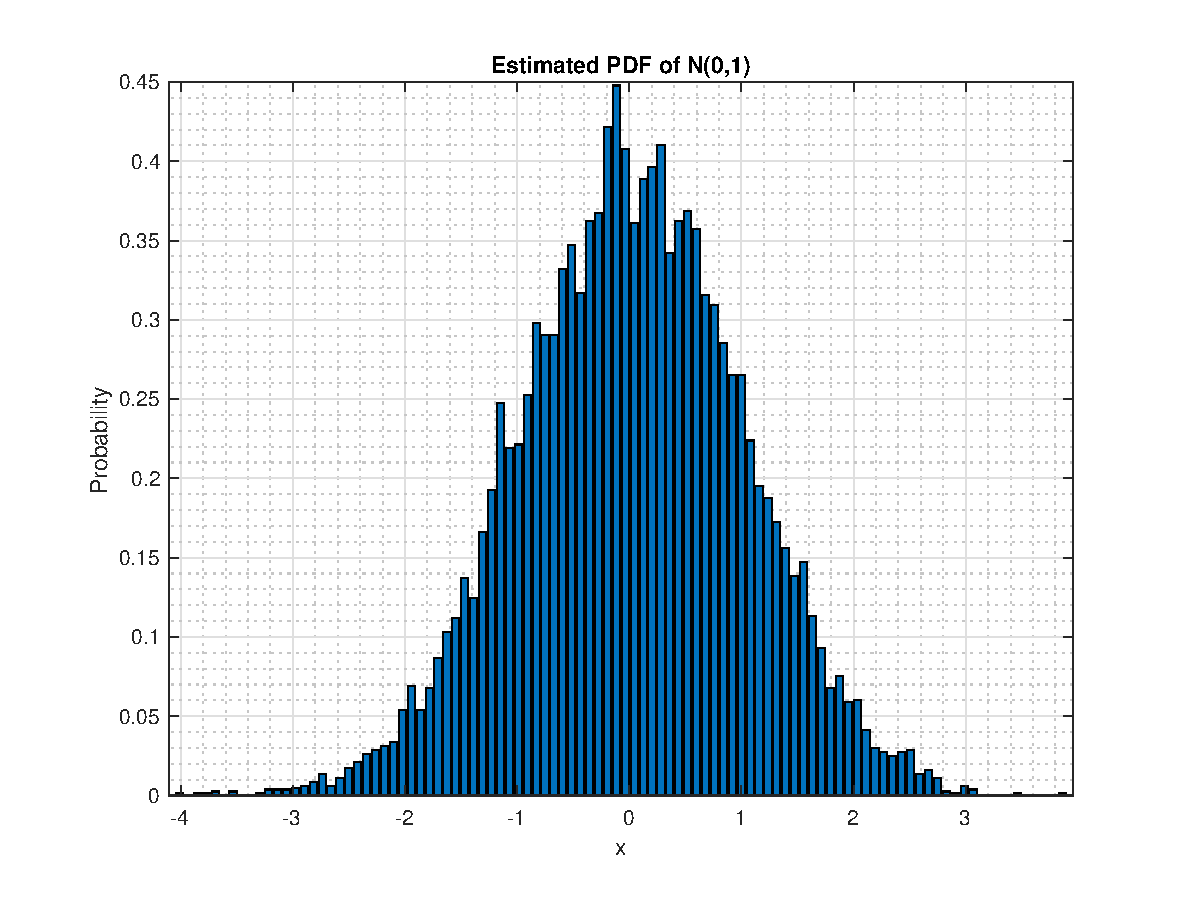
\includegraphics[width=0.5\textwidth]{pdf}
\caption{\label{fig:pdf} Estimated PDF for 10,000 samples of $N(0,1)$ using improved technique}
\end{figure}


\pagebreak


\subsubsection{For a stationary and ergodic process}

We analyze $rp3$ since it is the only signal that is both stationary and ergodic. We can clearly see in Figure \ref{fig:pdf_stat} that the matching between theoretical and estimated values increases with a greater number of samples.

\begin{figure}[h!]
\centering
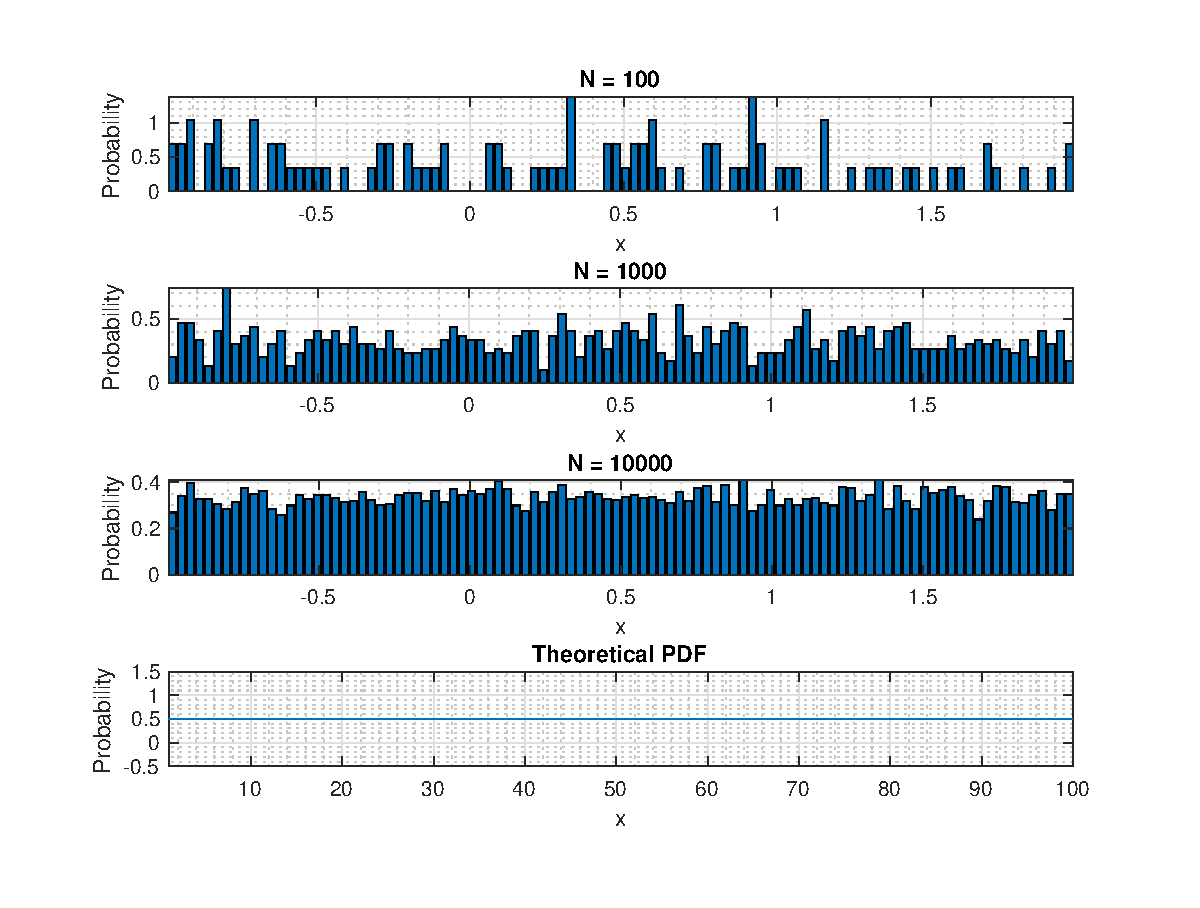
\includegraphics[width=0.7\textwidth]{pdf_stat}
\caption{\label{fig:pdf_stat} Comparing theoretical and estimated PDF of $rp3$}
\end{figure}


\subsubsection{For a non-stationary process}

The estimated PDF, shown in Figure \ref{fig:pdf_nonstat}, incorrectly tells us that $rp2$ is a random number between $1$ and $20$. We know that $rp2$ is not stationary since it is linearly increasing with time, and therefore our program causes loss of critical information about the signal. It is worth noting that stationary processes would not contain this kind of data.

\begin{figure}[h!]
\centering
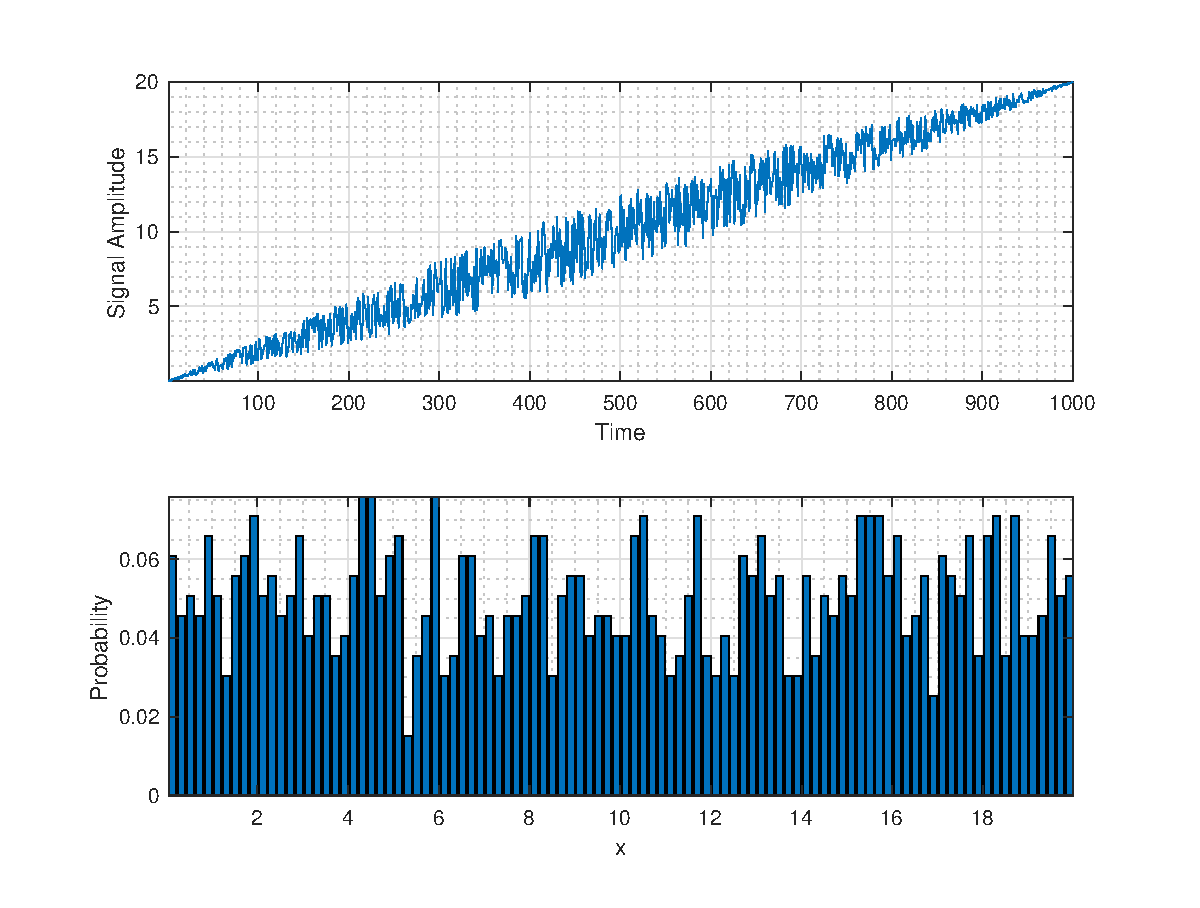
\includegraphics[width=0.7\textwidth]{pdf_nonstat}
\caption{\label{fig:pdf_nonstat} The signal $rp2$ and its estimated PDF}
\end{figure}


%\end{document}